%\section*{Collaborators}
%List all your collaborators.

\documentclass[11pt]{article}

\usepackage[margin=1in]{geometry}
\usepackage{amsmath,amsthm,amssymb}
\usepackage{color}
\usepackage{lipsum} % for filler text
\usepackage{fancyhdr}
\usepackage{graphicx}
\graphicspath{ {images/} }
\pagestyle{fancy}
\usepackage{enumitem}

\newenvironment{problem}[2][Problem]{\begin{trivlist}
\item[\hskip \labelsep {\bfseries #1}\hskip \labelsep {\bfseries #2.}]}{\end{trivlist}}

\fancyhead{} % clear all header fields
\renewcommand{\headrulewidth}{0pt} % no line in header area
\fancyfoot{} % clear all footer fields
\fancyfoot[LE,RO]{\thepage}           % page number in "outer" position of footer line
\fancyfoot[RE,LO]{Aashish Dhakal} %your name in footer line

\begin{document}
%\lipsum[1-20]
\title{CS 572(Assignment 2)} %replace X with the appropriate number
\author{Aashish Dhakal\\ %replace with your name
aashish@iastate.edu\\%replace with username
 }      %if necessary, replace with your course title
\date{}


\maketitle
\section*{}

\textbf{Problem 3.6)d)}
\\ States: Any combination of filled or empty jugs i.e. $[a, b, c]$\\
Inital State: Jugs have Value [0, 0, 0] i.e. all jugs are empty \\
Goal State: Values of jugs are $[a, b, c]$ where one of $a, b, c$ have value 1\\
Successor function: Given $[a, b, c]$ generate:\\
$[0, b, c]$, $[a, 0, c]$, $[a, b, 0]$  (empty into drain)\\
$[a-min(a+b,8)+b, min(a+b,8), c]$ (empty a into b)\\
$[a, b-min(b+c,3)+c, min(b+c,3)]$ (empty b into c)\\
$[min(a+c,12), b, c-min(a+b,12)+a]$ (empty c into a)\\
$[a-min(a+c,3)+c, b, min(a+c,3)]$ (empty a into c)\\
$[min(a+b,12), b-min(a+b,12)+a, c]$ (empty b into a)\\
$[a, min(b+c,8), c-min(b+c,8)+b]$ (empty c into b)\\
Cost Function: Number of actions \\ \\
\textbf{Problem 3.9}
\\ State: $[M, C, D]$ which gives the number of Missionary, Cannibal and the Side where the boat is.\\
a) The diagram of the complete state space is: \\
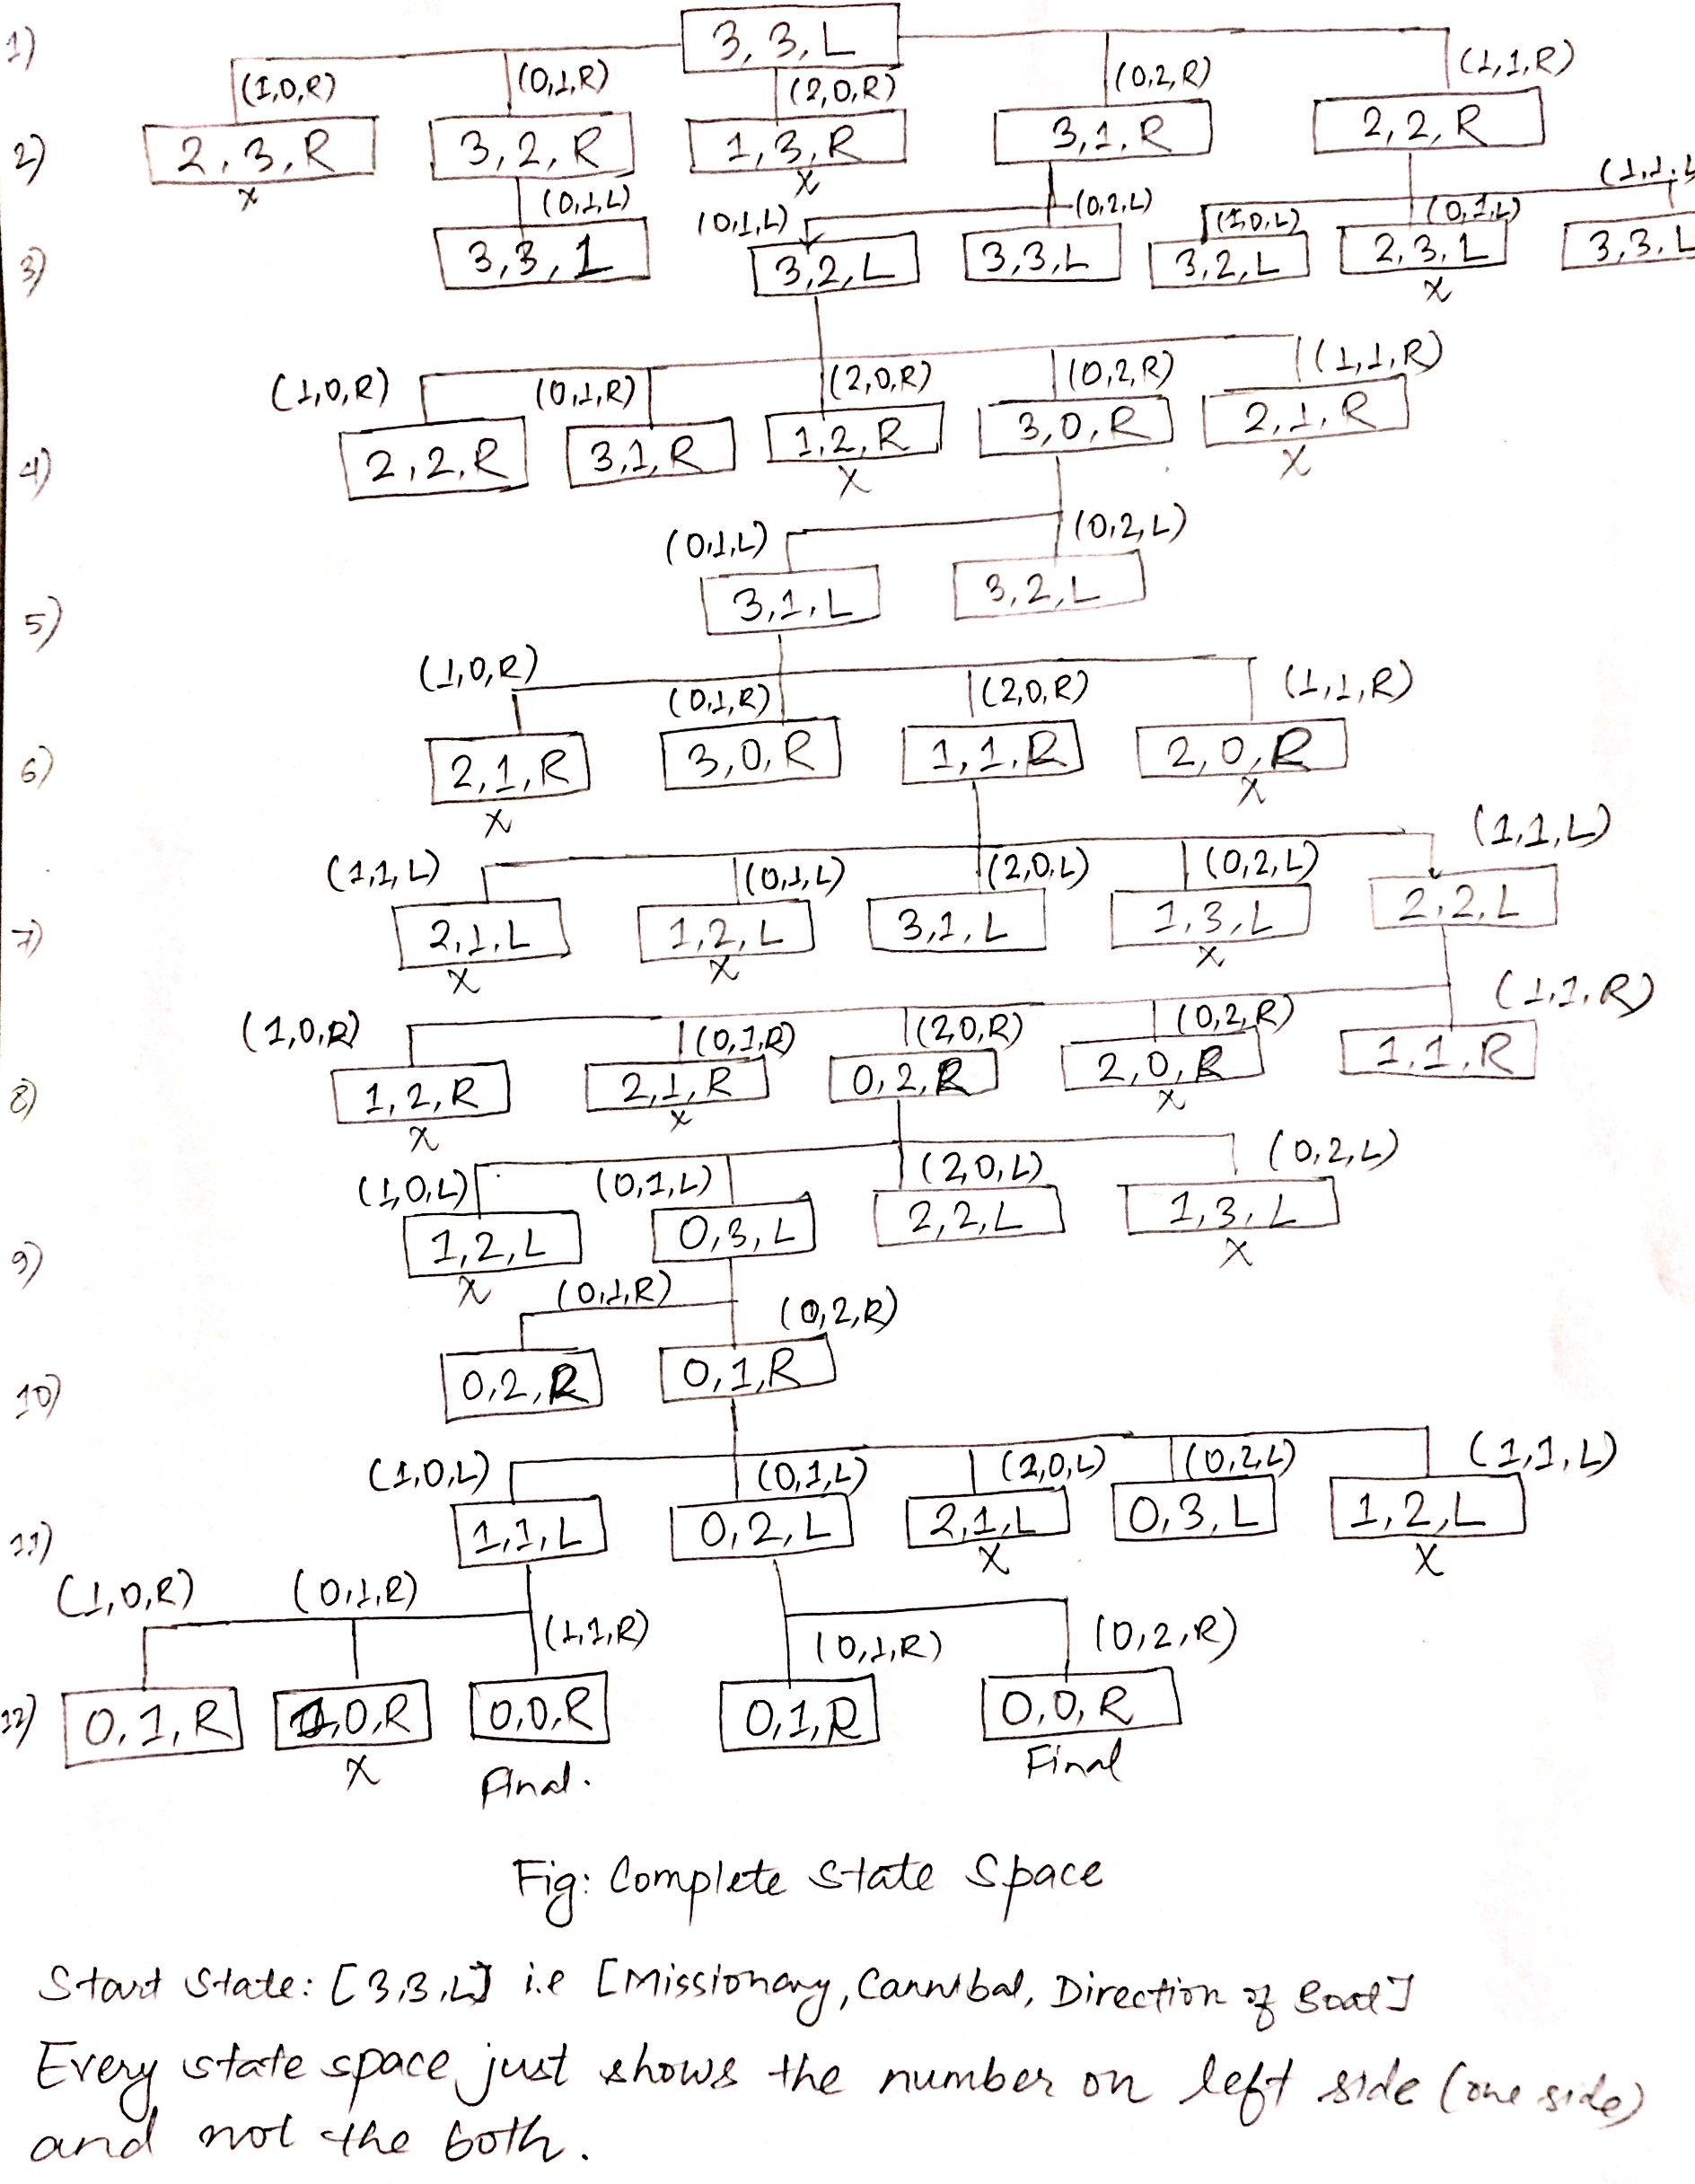
\includegraphics[width=150mm]{a.jpg}\\
b) We use the DFS to solve the problem optimally. We branch down one path and see if it gets to the solution or not. If it does not, we come back to the root
node and start exploring the other children. When we encounter repeated states, we ignore the current repeated states and move to other child node.
Yes, it is a good idea to check for the repeated states because we might get stuck in a loop.\\
The diagram for solution is:\\
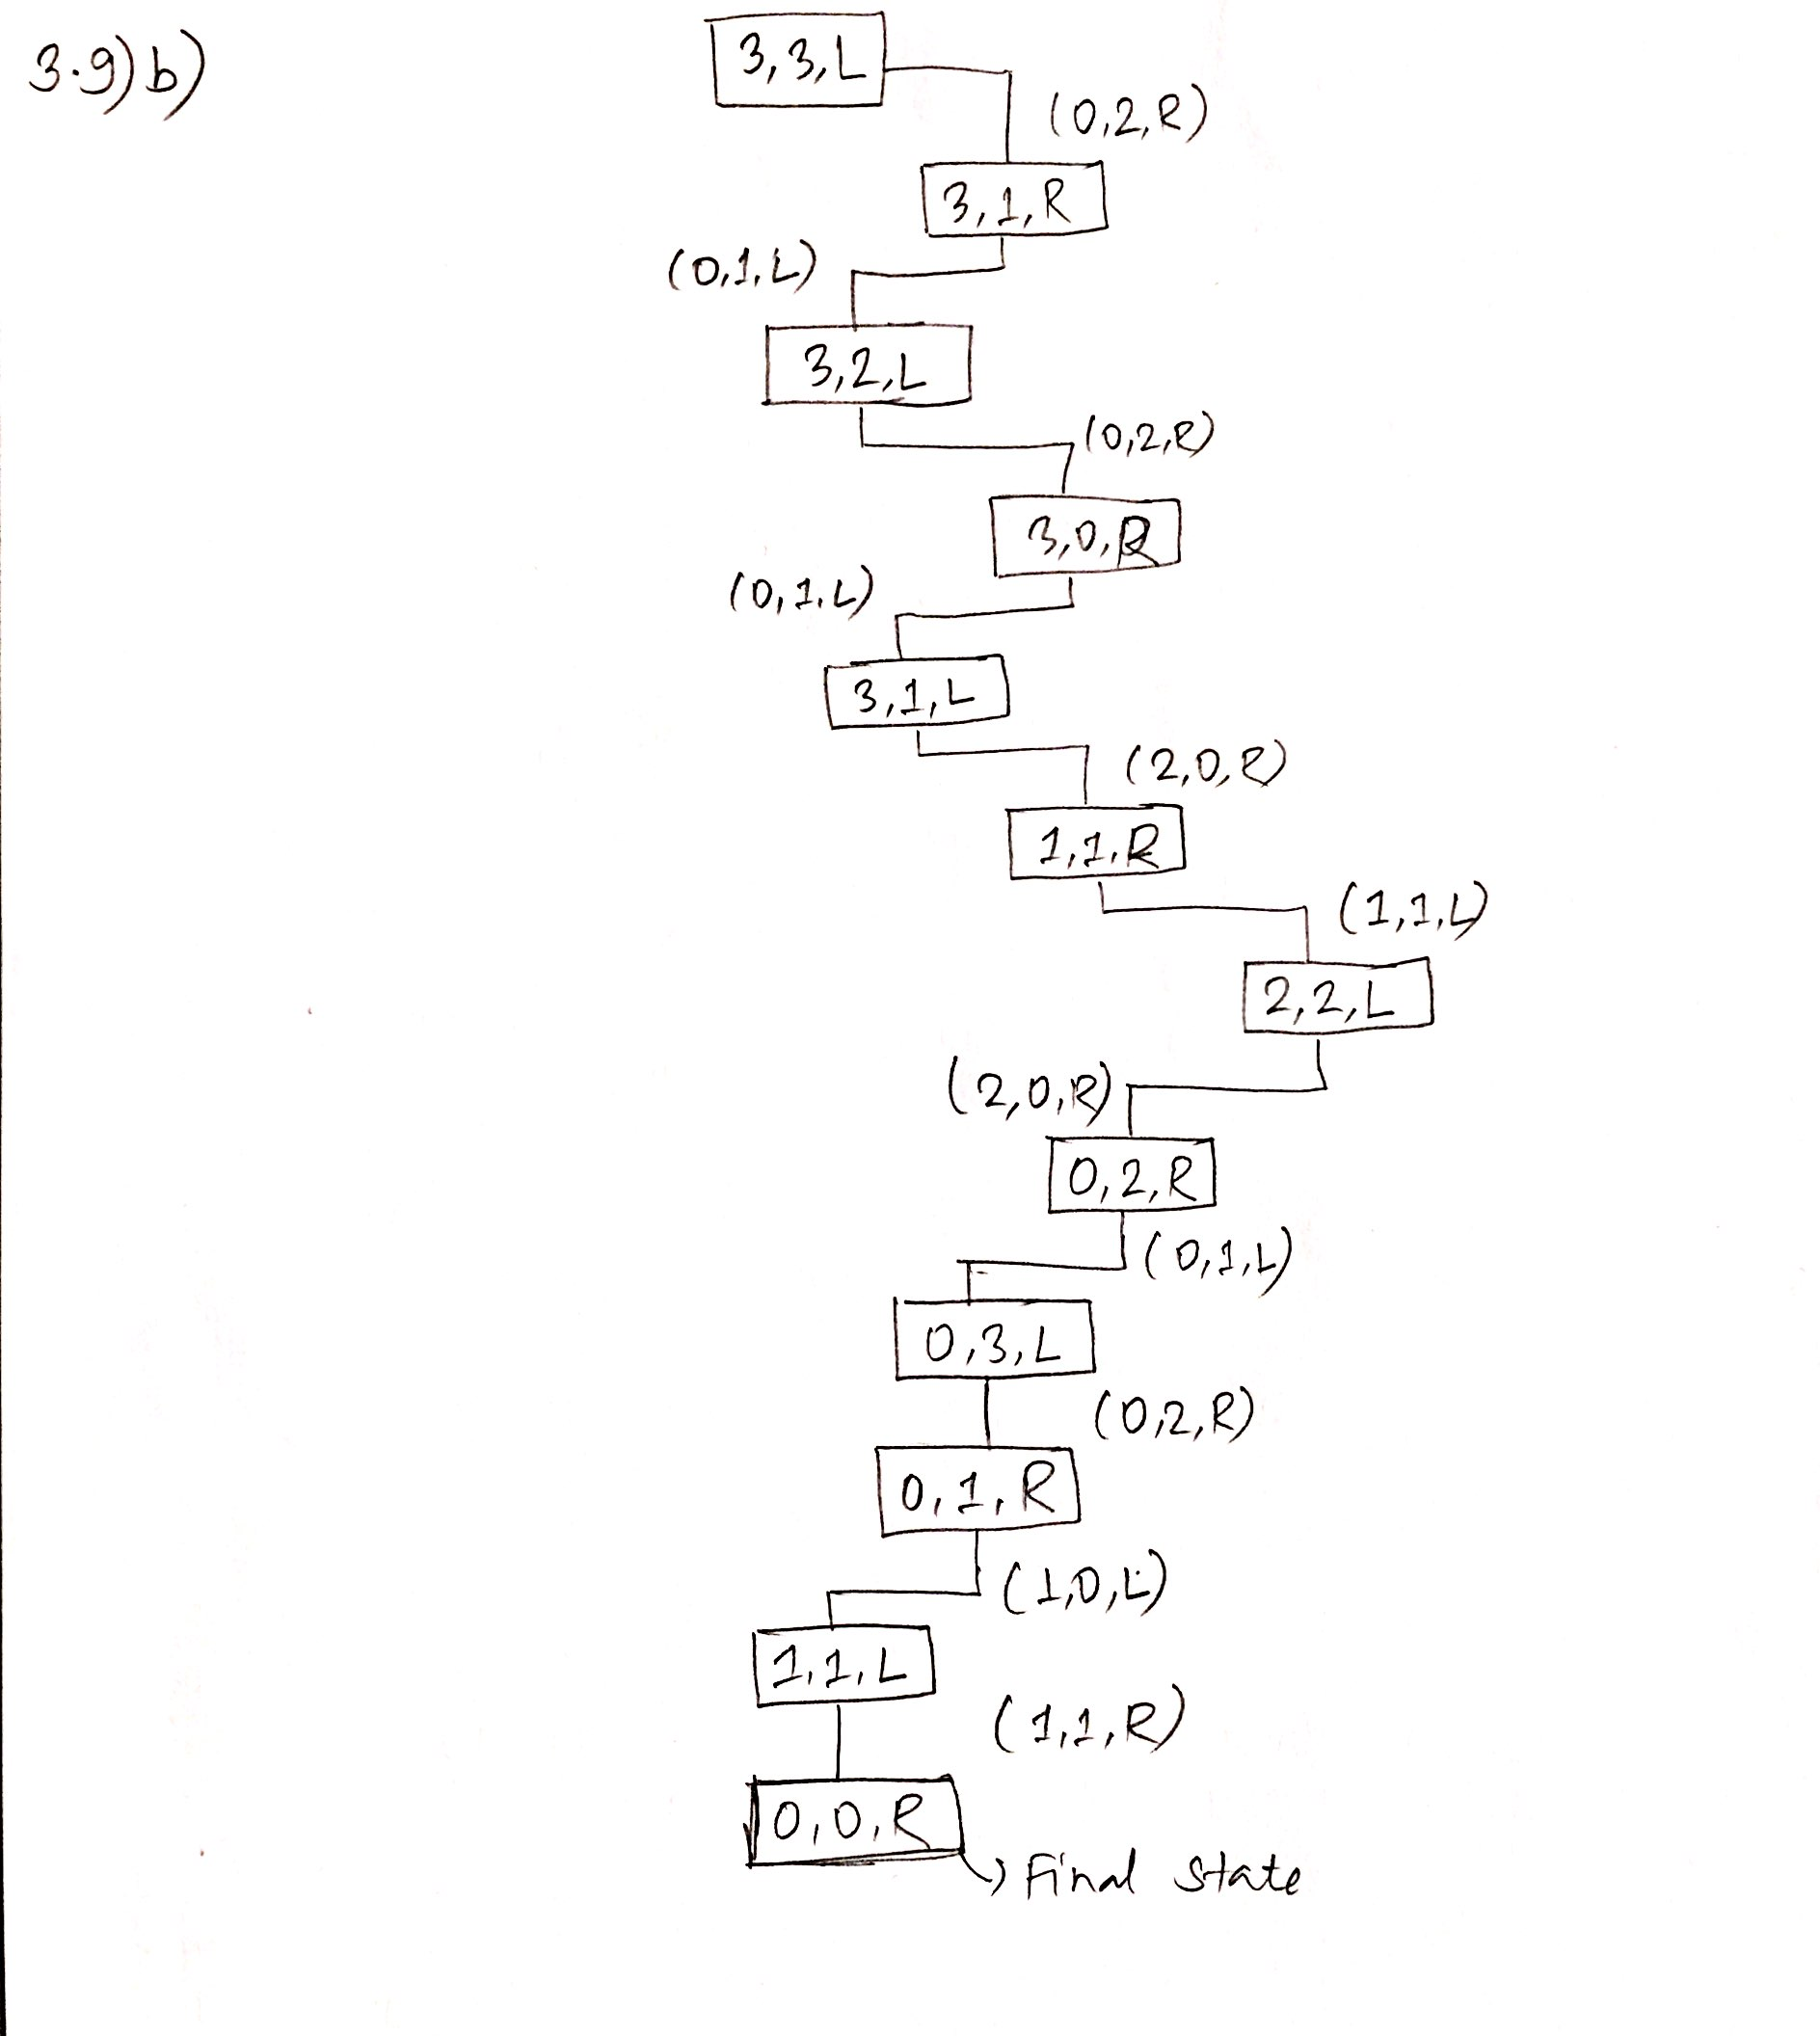
\includegraphics[width=150mm]{b.jpg}\\
c) Since, we don't have much idea about the future states, like if it's going to be repeated in future or after some moves
it is going to have an illegal state or not, it ends up in being a more complex problem.\\
\end{document}
}
